\documentclass[a4j,dvipdfmx]{jsarticle}

\usepackage[dvipdfmx]{graphicx}
\usepackage{amsmath,amssymb}
\usepackage{siunitx}
\usepackage{ascmac}
\usepackage[subrefformat=parens]{subcaption}
\usepackage{fancyhdr}
\usepackage{otf}
\usepackage[dvipdfmx]{hyperref}
\usepackage{pxjahyper}
\usepackage{okumacro}
\usepackage{tikz}
\usepackage{bm}
\usepackage{ulem}

\usepackage{titlesec}
\usepackage{tocloft} % 目次の設定をカスタマイズするためのパッケージ

% 式番号専用のセクション番号(「\S」を除外)
\newcommand{\plainsectionnumber}{\arabic{section}}

% 式番号にセクション番号を反映
\numberwithin{equation}{section}
\renewcommand{\theequation}{\plainsectionnumber.\arabic{equation}}

\pagestyle{headings}

% \renewcommand{\thesubsection}{\arabic{subsection}}
\renewcommand{\headrulewidth}{1pt}
\renewcommand{\Re}{\operatorname{Re}}
\renewcommand{\Im}{\operatorname{Im}}

% 目次にも「\S」を反映
\renewcommand{\thesection}{\S\arabic{section}}

% tocの番号幅を調整(「\S」で番号が長くなるため)
\setlength{\cftsecnumwidth}{3.5em} % セクション番号の幅を調整



\newcounter{basic_quastion}\setcounter{basic_quastion}{1}
\newcommand{\basicquestion}{\noindent{\large 基本問題\hspace{1mm}\huge\fbox{\textbf{\arabic{basic_quastion}}}\addtocounter{basic_quastion}{1}}\thispagestyle{fancy}\lhead{$\Sigma$基本問題}\rhead{\thepage}\cfoot{}\quad}
\newcommand{\sign}{\mathop{\mathrm{sign}}\nolimits}
\newcommand{\linktoMOKUZI}{\vspace{\stretch{1}}\fbox{\centerline{\hyperref[目次]{目次に戻る}}}}

\newcounter{basic_answer}\setcounter{basic_answer}{1}
\newcommand{\basicanswer}{\noindent{\large 基本問題\hspace{1mm}\huge\fbox{\textbf{\arabic{basic_answer}}}\addtocounter{basic_answer}{1}}\thispagestyle{fancy}\lhead{基本問題解答}\rhead{\thepage}\cfoot{}\quad}

\title{Quuノート -微分積分\ajRoman{2}-}
\date{最終更新 2025/01/10}
\author{責任者 Quu}

\begin{document}
    \maketitle
        \thispagestyle{empty}
    \begin{figure}[h]
        \centering
        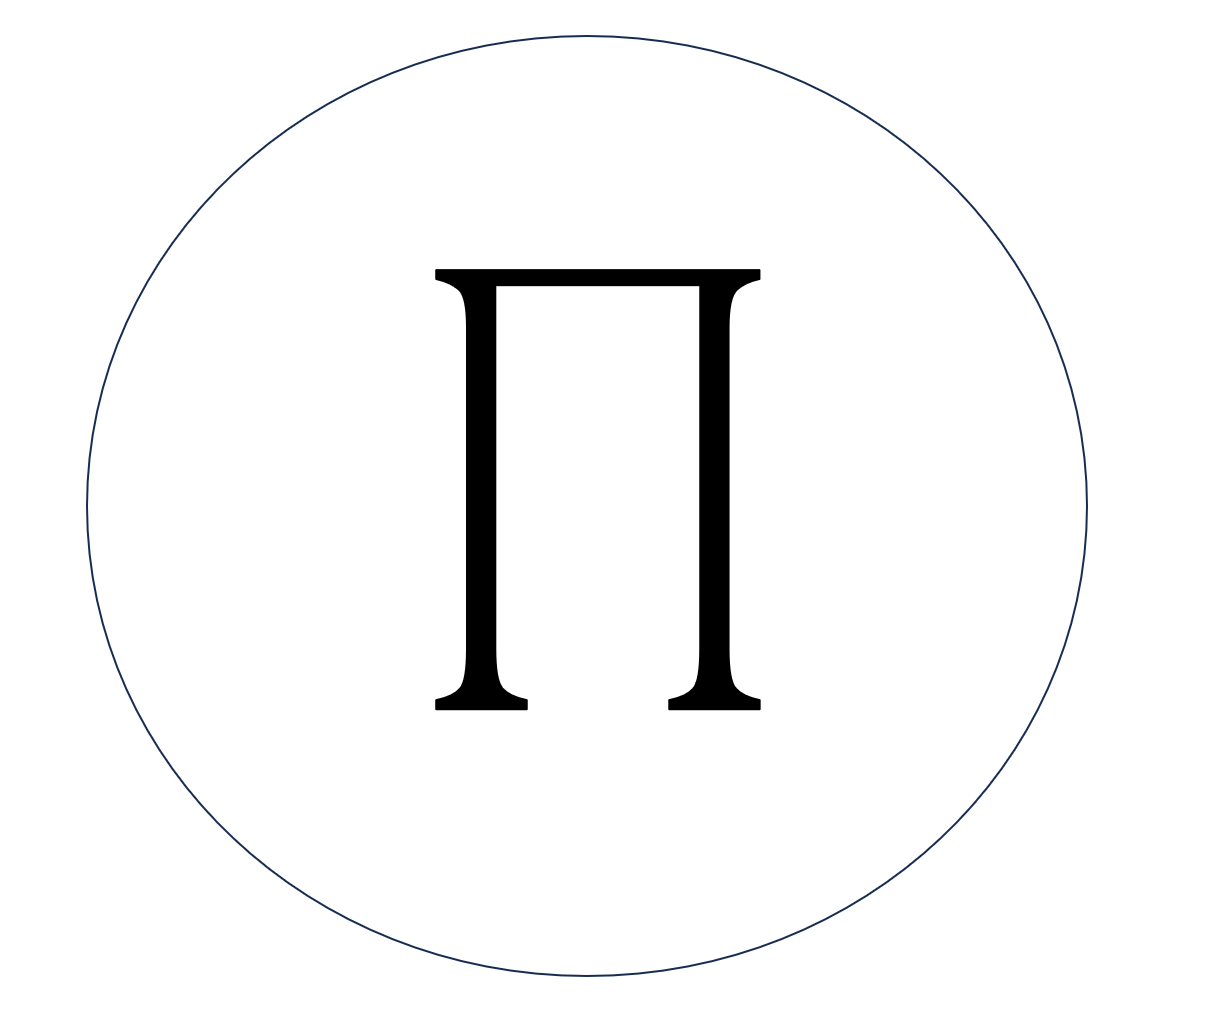
\includegraphics[scale=0.5]{img/QuuNote/QuuNote2/icon.png}
    \end{figure}
    
    \vspace{\stretch{1}}
    \centerline{\textbf{概要}}
    \noindent
    微分積分学入門についてのノート.\\
    主に, 多変数微分積分, ベクトル解析, 複素解析について扱う.
    \clearpage
     
    \clearpage
    \part*{このノートを読む前に}
        この本の読み方とか, この本が扱う内容について書く予定. 今回から英語人名にすることとか, 「.」や「,」を使うことも触れる.
    \clearpage
    \label{目次}
    \tableofcontents
    \clearpage

    \part{基礎数学}
    \vspace{\stretch{1}}
    \begin{screen}
        ここでは, 数学をするうえで必要となる最低限の基礎知識を学ぶ. 主に, 集合論基礎, 線形代数のうちベクトル, 行列, 行列式の基礎が含まれる.
        また, 多変数関数について微分・積分を定義する. いわゆる偏微分, 重積分というもので, これらの概念を習得することは, 数学, 物理, 工学を学ぶ上で重要である.
    \end{screen}
    \clearpage
    \section{集合論基礎}
        集合とその演算, 写像, 濃度について軽く触れ, 実数論についても少し触れる.
        \subsection{集合とは}
            \textbf{集合}とは端的に言えば, \underline{ものの集まり}である. 実数の集まりでも整数の集まりでもよいし, 関数の集まりでもよい.
            もっと具体的に, 犬, 猫, 人間, など, ともかく何かを集めた集まりである. ある集合に対して, あるものがその集合に含まれていた場合, 
            そのものを集合の\textbf{要素}や\textbf{元}という. 集合を構成するものといってもよいだろう. $a$が集合$A$の要素であることを次のように表記し, $a$
            は$A$に属するという.
            \begin{equation}
                a \in A \text{または} A \ni a \label{eq:集合論基礎:元の表記}
            \end{equation}
            また, $a$が$A$の要素でないことは$a\not\in A$または$A \not\ni a$と表記する. 例えば, $A$が6の約数全てであるとき, 
            $1\in A,2\in A$であるが, $5\not\in A$である. なお, 集合が集合たるためには, その集める範囲が明確に定義できていなければならない.
            例えば, 学校内の美人な学生全体の集まりは, 美人の定義が定まっていないから集合ではないのである. 大きい服すべての集まり, おいしい食べ物全体の集まり
            なども同様の理由で集合ではない. \\
        
            集合はものの集まりであるから, その要素の個数について気になるところである. 要素の個数が0か自然数で表せる集合を\textbf{有限集合}といい, 
            それ以外の集合を\textbf{無限集合}という. また, 要素の個数が0, すなわち要素を何も持たない集合を\textbf{空集合}といい, $\varnothing$とかく.
            有限集合としては例えば先ほど例に挙げた6の約数全ての集合がある. 無限集合としては, 自然数全体の集合, 実数全体の集合などがある.

            様々な集合を考えることができるが, 特別な記号で表せる集合があるから紹介しておこう. これらは一般的に, たいてい断りなく用いられる.
            \begin{align*}
                \mathbb{N}&=\text{自然数全体の集合}\\
                \mathbb{Z}&=\text{整数全体の集合}\\
                \mathbb{Q}&=\text{有理数全体の集合}\\
                \mathbb{R}&=\text{実数全体の集合}\\
                \mathbb{C}&=\text{複素数全体の集合}\\
            \end{align*}
            集合を表す方法として, その要素をすべて書き並べる表し方がある. これを\textbf{列記法}または\textbf{外延的記法}という.
            これを用いて, 先ほど例示した6の約数全ての集合を表す.
            \begin{equation}
                A=\{-6,-3,-2,-1,1,2,3,6\} \label{eq:集合論基礎:列記法の例}
            \end{equation}
            もちろん, 元を書き並べる順序をかえても同じ集合である. また, 重複して書かれた要素は一つのものとして考え, 同じ要素を重複して書くようなことはしない.
            しかし, 要素の数が多くなれば, 要素を全て並べて書くことは困難になることは容易に想像できる. 例えば100万以下の自然数すべての集合を列記法でかく作業は途方もないだろう.
            そこで, 集合の要素となる条件(範囲, 性質)を書いて, それを満たす要素全体として集合を表す方法も存在する. これを\textbf{説明法}や\textbf{内包的記法}という.
            これを用いて先ほどの\eqref{eq:集合論基礎:列記法の例}を書くと
            \begin{equation}
                A=\{x\mid\text{$x$は6の約数全体}\} \label{eq:集合論基礎:説明法の例}
            \end{equation}
            となる. このように, 説明法では集合を要素$x$の条件$P(x)$を用いて$\{x\mid P(x)\}$とかく. また, \eqref{eq:集合論基礎:説明法の例}は$\{x\in\mathbb{Z}\mid\text{$x$は6の約数全体}\}$
            とも書かれる. 最初の$x$の前に大前提の$x\in\mathbb{Z}$を書くのである. このほかにも, 特別な集合の場合は固有の表し方もある. 例えば, 閉区間, 開区間の表し方がそうである.\\

            義務教育中に習ったように, 自然数$\mathbb{N}$のすべての要素は整数$\mathbb{Z}$に含まれている. これは, $\mathbb{N}$が$\mathbb{Z}$に`包まれている'ような状態であると理解できる.
            一般に, 二つの集合$A,B$について, $A$の\underline{全ての}要素が$B$の要素であるとき, $A$は$B$の\textbf{部分集合}であるといい,
            \begin{equation}
                A \subset B \text{または} B \supset A \label{eq:集合論基礎:部分集合の表記}
            \end{equation} 
            とかく. この場合, $A$は$B$に\textbf{包まれている}, または$B$は$A$を\textbf{包む}という. 反対に, $A\subset B$ではないことを$A\not\subset B$とかく.
            明らかに, $A\subset A$である. また, $A\subset B,B\subset C$ならば$A\subset C$であることも, 明らかであろう. 
            $A\subset B$かつ$A \supset B$であるとき, $A=B$とかき, 二つの集合$A,B$は\textbf{等しい}という.

            $A\subset B$かつ$A\neq B$であるとき, $A$は$B$の\textbf{真部分集合}であるといい, これを強調したい時$A\subsetneq B$とかく. 例えば, $\mathbb{N}$は$\mathbb{Z}$
            の真部分集合である.\\

            集合$A$に対して, $A$の部分集合全体の集合を$A$の\textbf{巾集合}といい, $\mathfrak{P}(A), \mathcal{P}(A), 2^{A}$のようにかく.本ノートでは, 最後の記法$2^{A}$を採用することにする.
            巾集合は, その要素全てが集合である. 一般に, どの要素も集合であるような集合を\textbf{集合族}という.\footnote{集合族は, 一般にドイツ文字や花文字で表される慣習がある.}

            例えば, $A=\{1,2,3\}$のとき$2^{A}=\{\varnothing,\{1\},\{2\},\{3\},\{1,2\},\{1,3\},\{2,3\},\{1,2,3\}\}$である. 空集合が入っていることに疑問が浮かぶ人もいるだろうから説明しておこう.
            空集合とは, 要素を一つも持たない集合であるから, 論理として「$a$が$A$に含まれていない」ならば「$a$は$\varnothing$に含まれていない」が任意の集合$A$に対して成り立つ.
            実際, 前半の「」の真偽にかかわらず成り立つから, これは正しいと納得されるだろう.\footnote{これは次小節を見ることでより納得がいくはずである.} 
            このときこの命題の対偶\footnote{次小節参照.}を取れば, 「$a$が$\varnothing$に含まれている」ならば「$a$は$A$に含まれている」が成り立つ.
            すなわち, 空集合は任意の集合の部分集合であることがわかる. 
        \clearpage
        \subsection{記号論理}
    \clearpage
    \section{行列と行列式}
        ベクトルのイメージとその和・差について. 内積についても述べる. 外積はベクトル解析のときに述べる. 続いて, 行列についてその定義を述べ, 和・差・積について述べる.
        転置行列と逆行列についても述べる. 行列式は, 一般の定義を述べ, その後2x2と3x3について計算方法を述べる. 余因子展開についてその計算方法を述べる.
    \clearpage
    \section{偏微分}
        多変数関数をまず具体例で挙げ, その後偏微分について解説する.二変数テイラー展開及び積分記号下の微分まで述べる.
    \clearpage
    \section{多重積分}
        多重積分についてまず二重積分についてその定義を話す. かんたんな計算ののちに三重積分も述べる. その後, 変数返還について, 一次変換の場合について厳密な証明を行い, 
        それ以外は感覚的なものにとどめる.
    \clearpage
    
    \part{ベクトル解析}
    \vspace{\stretch{1}}
    \begin{screen}
        ベクトル解析は, 理工系の学生にとって馴染み深いものと聞く. たいていの物理科と電気科の学生は, 電磁気学にて顔を合わせることになるだろう.
        よく電磁気学は, ベクトル解析をふんだんに用いるから難しいと言われているが, 少なくともベクトル解析単体で見ればそこまで難しいものではない. 
        そして何よりベクトル解析は楽しいものである. ここでは, まずベクトルについての基礎知識について述べた後, ベクトル値関数についてその微分積分を定義する.
        その後, 空間上の曲線および曲面の解析についてすこし述べ, ベクトル解析の顔ともいえる微分演算子について述べる.
        電磁気学ではよく用いられるGaussの発散定理およびStokesの定理についても扱う. 
    \end{screen}
    \clearpage
    \section{ベクトルの性質と演算}
        数学基礎で述べたことと多少重複するが, 内積, 外積およびそれらの性質を述べる. スカラー三重積とベクトル三重積も述べる.
    \clearpage
    \section{ベクトル値関数とその微分}
        ベクトル値関数について述べたのち, それらの微分積分を定義する. ただし, 積分は定義のみで深く触れない.
    \clearpage
    \section{曲線の解析}
        曲線について解析する. 平面曲線について述べて, 空間曲線でも議論する. Frenet-Serretの公式まで.
    \clearpage
    \section{曲面論入門}
        曲面について解析する. 基本量を導出し, Gauss曲率と平均曲率を紹介する.
    \clearpage
    \section{微分演算子}
        ベクトル場とスカラー場について説明する. その後各微分演算子について述べる.
    \clearpage
    \section{線積分と面積分}
        線積分と面積分について定義を述べる. Gaussの定理とStokesの定理について述べ, 電磁気学への応用をしてみる.
    \clearpage

    \part{複素解析}
    \vspace{\stretch{1}}
    \begin{screen}
        複素解析は, 数学の中で最も美しい理論の一つと言われる. 複素関数(複素数から複素数へ対応させる関数)に対して, 正則という概念が定義できる.
        正則性とはかんたんに言えば微分可能性のことなのであるが, 驚くべきことにこの正則性を満たせば,それらを微分した関数も正則性を保つのである. 
        これらの性質を含め, 正則関数の解析の基本となるのはCauchyの積分定理である. ここでは, 複素数についてその基本的な性質を述べ, 複素関数および
        複素微分について定義し, 複素平面上での積分を述べる. その後, Cauchyの積分定理をはじめとする, 正則関数に関する多くの定理を証明する.
        その中には実積分の計算に対してたいへん有効な留数定理もある. この理論の美しさをじっくり味わってほしい.
    \end{screen}
    \clearpage
    \section{複素数}
        複素数についてその基礎知識を述べる. 複素平面上の領域も. De Moivreの定理まで述べる.
    \clearpage
    \section{複素関数とその微分}
        複素関数について定義し, その性質について簡単に述べる. Cauchy-Riemannの方程式も述べる. 初等関数についても述べる.
    \clearpage
    \section{複素線積分}
        かんたんな線積分の計算をして, Cauchyの積分定理を述べる. Cauchyの積分公式やGoursatの定理などの多数定理を述べる. 最大値の原理
        については証明させる?
    \clearpage
    \section{級数}
        複素数列について, その収束等を定義し, 複素級数についても定義する. ベキ級数やTaylor展開, Maclaurin展開についても述べる.
        Laurent展開を重点的に扱う.特異点とその分類も述べる.Picardの大定理は入れない. 無限遠点のLaurent展開も述べる.
    \clearpage
    \section{留数定理}
        留数について定義を述べて, 留数定理を示す. その後, 実積分の計算を行う. 無限遠での留数についても述べる.
    \clearpage
    \section{解析接続}
        解析接続について簡単な例を挙げ, 一致の定理を証明して, 解析接続の一意性について説明する.
    \clearpage
    \section{Riemann面}
        余裕があれば,多価関数とRiemann面についてすこしだけ述べる.
    \clearpage

    \part{相対性理論}
    \vspace{\stretch{1}}
    \begin{screen}
        相対性理論...それはかの天才物理学者Einsteinが作り上げた物理学の中で最も美しい理論である. 理科や宇宙が好きな
        小学生であればほとんどの人があこがれていたものであると思うし, それ以外の人でも, 相対性理論から導かれる不思議な
        世界(双子のパラドクスなど)について聞いたことがある人も多いと思う. 相対性理論が美しいといわれるその所以は, たった一つ
        の物理的要請に真摯に従って計算することで, 重力場の基礎方程式(いわゆる, Einstein方程式)までたどり着けるところであろう. 
        その要請とは, 「物理学の法則は, 座標系に依存しない形式に書かれなければならない」という, 実に自然な, 当然ともいえる要請である.
        この要請から, さまざまな相対性理論の世界が開けることには, ただただ驚嘆するばかりである.\\
        相対性理論は, 一般に非常に難しいといわれている. 確かに, 相対性理論, 特に一般相対性理論を真に理解するには, 数学のRiemann幾何学について熟知していないといけないだろう.
        しかし, 特殊相対性理論に限って言えば, かんたんな力学の知識さえあれば(一部を除いて)理解することができる. また, 一般相対性理論に関しても, 重力場の方程式を導くだけであれば
        必要なRiemann幾何学の知識も特別難しいものではないのである.\\
        ここでは, 特殊相対性理論について, よく子供向けの科学本などに載っている事象を中心に数学的に理解していく.
        また, 一般相対性理論についても軽く触れる.
    \end{screen}
    \clearpage
    \section{特殊相対論入門}
        Galilei変換についてと慣性系について述べる. 光速度不変の原理について, 実験結果から述べ, Lorentz変換を導出する. 
         Minkowski時空上の距離, 世界間隔について説明する. このときLorentz変換に対して不変であることを述べる.
        固有時間などについても述べる.
    \clearpage
    \section{パラドクスの解決}
        パラドクスをここで解決する. 双子のパラドクスと時計のパラドクス
    \clearpage
    \section{数学的準備}
        ベクトルやテンソルについて, かんたんに定義する.
    \clearpage
    \section{相対論的力学}
        相対論上で力学を展開する. $E=mc^2$の導出や変分原理についても扱う. 双子のパラドクスを変分原理を用いて解決する.
    \clearpage
    \section{一般相対論への展望}
        Riemann幾何学の$ds^2$を紹介して, 等価原理について$\Gamma=0$であることを紹介する.
    \clearpage

    \part{Lebesgue積分入門}
    \vspace{\stretch{1}}
    \begin{screen}
        積分好きなら一度は聞いたことがあるのが, このLebesgue積分である. Lebesgue積分は, 単なる数学の枠を飛び越えて, 
        物理学や工学で必須のFourier解析や, 偏微分方程式, また確率論などのいたるところに顔を出す非常に重要な概念である.
        それにもかかわらず, このLebesgue積分はなかなかに難しく, 習得にも時間がかかる. これはLebesgue積分が素朴なRiemann積分と違って
        内容がいささか抽象的であることが原因であるように思える. さらに, 集合論に関する知識も必要であり, 学ぶための敷居が高い.
        そこでここでは, Lebesgue積分論のうち, 特に重要であるものを選択して系統的に学べるよう, 構成を工夫した. 
        端的に言えば, 極限と積分の順序交換ができる単調収束定理へ最短経路で学べるようになっているのである.
        なおこのLebesgue積分は, Riemann積分と対照的に, しばしばグラフを横に切る積分であると説明される. 実際まちがってはないが, 
        実際にLebesgue積分を学んでいると, 横に切っているというイメージはあまりないので注意してほしい.
    \end{screen}
    \clearpage
    \section{可測空間}
        集合体, $\sigma$-集合体の定義を述べ, 可測空間を定義する. 部分集合族から生成される$\sigma$-集合体や可測分割等も述べる.
    \clearpage
    \section{測度}
        集合関数の定義および測度の定義を述べる. 様々な測度の例を述べる. 測度の基本的な性質についても示す. $\mu$-零集合
        についても触れ, 完備測度空間を定義する. 完備測度への測度の拡張が存在し, しかもそれが一意であることを述べる.
    \clearpage
    \section{可測関数}
        可測関数の定義, 基本的性質を述べる. 単関数を定義し, 任意の正なる可測関数に対して, 収束する単関数の単調増加列が存在することを示す.
        ほとんど到る所(almost everywhere)についても触れる.
    \clearpage
    \section{積分}
        積分を定義し, 諸性質を述べる. 関数が連続であれば, Riemann積分とLebesgue測度に対する積分(Lebesgue積分)が一致することも述べる.
    \clearpage
    \section{収束定理}
        Lebesgueの有界収束定理を証明する. 適用例などをみてその威力を体感する.
    \clearpage
    \part{終わりに}

\end{document}